\documentclass{../beamer_template/myBeamer}

\input{../beamer_template/header.tex}

\title[Spatial sensitivity]{Spatial sensitivity analysis}
\subtitle{Course and practical application}
\author[Short Author]{Author}
\date{\today}
\institute{Institut\\
\bigskip
\includegraphics[scale=2]{../beamer_template/figures/logos/openmole.png}}

\begin{document}



\begin{frame}[plain]
	\titlepage
\end{frame}
\addtocounter{framenumber}{-1}

\AtBeginSection[]
{
	\frame{
		\tableofcontents[currentsection, hideallsubsections]
	}
	\addtocounter{framenumber}{-1}
}


\sframe{Outline}{
\tableofcontents
}



\section{Introduction}

\sframe{Context}{

\textit{Classical problems in geography and spatial sciences :}

\medskip

\begin{itemize}
	\item Modifiable Areal Unit Problem
	\item Dependancy to scale of processes
	\item Spatial non-stationarity
	\item Fuzzy and noisy data
	\item Genericity/particularity 
\end{itemize}

}



\sframe{Approach proposed by OpenMOLE}{

$\implies$ \textbf{spatial configuration are parameters too}

\medskip

\begin{itemize}
	\item ``\textit{Space matters}'': impact of spatial configuration on model behavior
	\item Model behaviors which are robust to spatial configuration
	\item Model behaviors which are robust to noise in parametrization real datasets
\end{itemize}

% - Space matters
% - Synthetic generators
% - Sensitivity to data noise
 
}



\sframe{Contents of this module}{

 %- Generation of spatial synthetic data
 %    - microscopic scale (buildings)
 %    - mesoscopic scale (population grid)
 %    - macroscopic scale (system of cities)
 %- Perturbation of real datasets
 %- Spatial indicators for model outputs
 %- Practice

	\tableofcontents

}



\section{Spatial synthetic data}



\sframe{General context}{

\justify

$\rightarrow$ coupling models with spatial configuration generators (spatial synthetic data) gives model sensitivity to space through sensitivity analysis of the coupled model

\bigskip

$\rightarrow$ synthetic urban forms resembling real configurations

\bigskip

$\rightarrow$ at different scales: microscopic (buildings), mesoscopic (population distribution), macroscopic (system of cities)

}



\sframe{Generating building layouts}{

\textit{At the microscopic scale (district): generating building layouts}

\nocite{raimbault2019generating}

\medskip

Raimbault, J. and Perret, J., 2019. Generating urban morphologies at large scales. \textit{Forthcoming in proceedings of Artificial Life 2019.} arXiv:1903.06807

\medskip

\begin{itemize}
	\item systematic comparison of simple processual generators
	\item introduction of morphological indicators
	\item calibration on sampled layouts from OpenStreetMap
\end{itemize}

}


\sframe{Quantifying urban form}{

% Simple descriptive indicators considered are (i) the total building density $A = \frac{1}{N}\cdot \sum_i s_i$; (ii) the number of buildings given by the number of connected components of $B$; (iii) the average building area, i.e. the average size of $B$ connected components; (iv) Moran index capturing spatial autocorrelation (see \cite{raimbault2018calibration} for its definition in a similar setting), with a simple inverse distance weight function; (v) average distance between non-empty points (which also captures a level of concentration).
% We also use indicators computed with the underlying networks: the average detour computed in the free space network $\bar{B}$, computed by randomly sampling 50 pairs of points in a connected component of $\bar{B}$ and computing the ratio between the network distance and the euclidian distance $d_{\bar{B}}/d_E$. This measures captures in a way the sinuosity of streets from a mobility viewpoint. We also consider the average size of open connected areas as the average size of the connected components of $\bar{B}$.
% steps for dilation + steps for erosion


}


\sframe{Generators}{

\textit{Complementary generators}

\medskip

\begin{center}
	\includegraphics[height=0.9\textheight]{figures/spatialsens_examplegenerators.png}
\end{center}


}

\sframe{Real configurations}{

\textit{Sampled districts from OpenStreetMap}

\medskip

\begin{center}
	\includegraphics[height=0.9\textheight]{figures/spatialsens_exampleosm.png}
\end{center}

}


\sframe{Classification of urban forms}{

\begin{center}
   \includegraphics[height=0.9\textheight]{figures/spatialsens_osm_classification.png}
\end{center}

}




\sframe{Calibrated forms}{

\centering

\includegraphics[width=\textwidth]{figures/spatialsens_calib.png}

}


\sframe{Point cloud}{


\includegraphics[height=\textheight]{figures/spatialsens_points.png}

}


\sframe{Calibration}{

\includegraphics{figures/spatialsens_distanceclasses.png}

\medskip

\textit{Why not calibrate ? Open question of fitting a point cloud}

}


\sframe{Implementation in OpenMOLE}{

% TODO spatialsmapling syntax 

}




\sframe{Synthetic population grids}{

\textit{At the mesoscopic scale: population grid}

\nocite{raimbault2018calibration}

\medskip




 - Reaction-diffusion model
 - Urban form measures


Raimbault, J. (2018). Calibration of a density-based model of urban morphogenesis. PloS one, 13(9), e0203516.

\nocite{raimbault2018calibration}

\smallskip

Raimbault, J. (2019). An urban morphogenesis model capturing interactions between networks and territories. In The Mathematics of Urban Morphology (pp. 383-409). Birkhäuser, Cham.

\nocite{raimbault2019urban}


}

\sframe{A simple Reaction-diffusion model}{


\justify

$\rightarrow$ Crucial role of the interplay between concentration forces and dispersion forces~\cite{fujita1996economics} in keeping Urban Systems at the border of chaos

\bigskip

$\rightarrow$ Potentiality of aggregation mechanisms (such as Simon model) to produce power laws %\cite{2016arXiv160806313S}

\bigskip

$\rightarrow$ Link with Reaction-diffusion approaches in Morphogenesis~\cite{turing1952chemical}

\bigskip

$\rightarrow$ Extension of a DLA-type model introduced by \cite{batty1991generating}, with simple abstract processes of population aggregation and diffusion

}


\sframe{Model Formalization}{

$\rightarrow$ Grid world with cell populations $(P_i(t))_{1\leq i\leq N^2}$.

\bigskip

$\rightarrow$ At each time step:

\begin{enumerate}
\item Population growth with exogenous rate $N_G$, attributed independently to a cell following a preferential attachment of strength $\alpha$
%\begin{equation}
%\Pb{P_i(t+1)=P_i(t)+1|P(t+1)=P(t)+1}=\frac{(P_i(t)/P(t))^{\alpha}}{\sum(P_i(t)/P(t))^{\alpha}}
%\end{equation}
%The attribution being uniformly drawn if all population are equal to 0.
\item Population is diffused $n_d$ times with strength $\beta$
\end{enumerate}

\bigskip

$\rightarrow$ Stopping criterion: fixed maximal population $P_m$.

%To avoid bord effects such as reflecting diffusion waves, border cells diffuse their due proportion outside of the world, implying that the total population at time $t$ is strictly smaller than $N_G\cdot t$.

\bigskip

$\rightarrow$ Output measured by morphological indicators: Moran index, average distance, rank-size hierarchy, entropy.


}


\sframe{Generating Population Distributions}{

\centering

\includegraphics[height=0.8\textheight]{figures/density_Fig2}

\footnotesize\textit{Examples of generated territorial shapes}

}


\sframe{Model behavior}{

% comment Arnaud : Les graphiques correspondent aux 4 exemples précédents ? Si oui les rappeler en petite vignette. -> NON

\centering

\includegraphics[width=0.9\textwidth]{figures/density_Fig3}

\footnotesize\textit{Phase transitions of indicators unveiled by exploration of the parameter space (80000 parameter points, 10 repetitions each)}

% comment Arnaud : Préciser (dimensionner)

}




\sframe{Path-dependence and frozen accidents}{

\centering

\includegraphics[width=0.8\textwidth]{figures/density_Fig4}

\footnotesize\textit{Illustration of path-dependence in a simplified one-dimensional version of the model: cell trajectories in time for 9 independent repetitions from the same initial configuration.}


}


\sframe{Empirical Data for Calibration}{


\begin{columns}
\column{0.6\textwidth}
\centering
\includegraphics[width=\textwidth]{figures/density_indics_morpho_discrquantiles}
\column{0.3\textwidth}
\centering
\includegraphics[width=\textwidth]{figures/density_cluster_pca_k5_morpho}\\
\includegraphics[width=\textwidth]{figures/density_cluster_map_k5_morpho}
\end{columns}

\justify

\footnotesize\textit{Computation of morphological indicators on population density data for Europe (shown here on France), morphological classification.}

}



\sframe{Model Calibration}{

\includegraphics[width=\textwidth]{figures/spatialsens_calibmorphogenesis}

\footnotesize\textit{Brute force calibration by exploring the parameter space. Reproduction of most existing configuration in the morphological sense (here in principal plan).}

}



\sframe{Model Targeted Exploration}{

\centering

\includegraphics[width=0.8\textwidth]{figures/spatialsens_pse.png}

\footnotesize\textit{Potentialities of targeted model explorations: here feasible space using Pattern Space Exploration algorithm \cite{10.1371/journal.pone.0138212}.}

}


\sframe{Generation of synthetic networks}{

% cite alife

}

\sframe{Coupled network-population generators}{

}






\sframe{Synthetic systems of cities}{


\textit{At the macroscopic scale: synthetic systems of cities}


\begin{itemize}
	\item Evolutive urban theory: systems of cities follow general stylized facts \cite{pumain2018evolutionary}
	\item Rank-size law \cite{pumain2006evolutionary}
	\item Central place theory
\end{itemize}


}

\sframe{Cities and networks}{

% simpopnet generator

}

\sframe{Co-evolution models}{

% ex from cities nw paper

}

\sframe{Other disciplines and spatial structures}{

% morphogensis : interdisc ?

% suggest: ecology (habitat / spatial niches ?) ; topography ; ?

}


\section{Perturbation of data}


\sframe{Real data perturbation}{

$\rightarrow$ \textit{How does noise in real data impacts the result ?}

% - WIP

\medskip

\begin{itemize}
	\item Impact of missing elements
	\item Impact of imprecise coordinates or topology
	\item Optimal matching between spatial datasets
\end{itemize}


\bigskip

$\rightarrow$ \textit{How does perturbation of real data allows to explore scenario}

An example: simulating urban projects by modifying population of areas with a given spatial correlation structure.
%Forcity example

}






\section{Application: sensitivity to spatial configuration}



\sframe{Method flowchart}{

\textit{General workflow to test the spatial sensitivity of simulation models}
% TODO cit spacematters

\centering

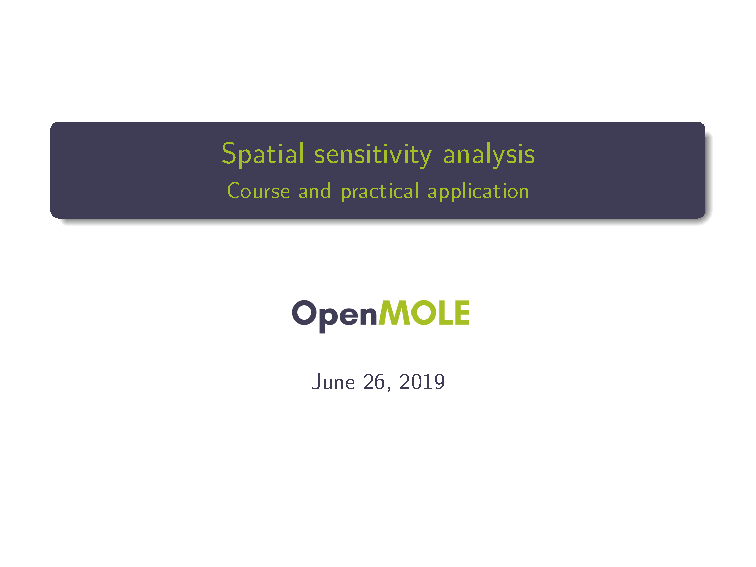
\includegraphics[width=\textwidth]{figures/spatialsens.png}

}


\sframe{Quantification of spatial sensitivity}{

\textit{Relative distance of phase diagrams to compare global model behavior when meta-parameters change}

\medskip

\[
d_r\left(\mu_{\vec{\alpha}_1},\mu_{\vec{\alpha}_2}\right) = 2 \cdot \frac{d(\mu_{\vec{\alpha}_1},\mu_{\vec{\alpha}_2})^2}{Var\left[\mu_{\vec{\alpha}_1}\right] + Var\left[\mu_{\vec{\alpha}_2}\right]}
\]

}


\sframe{Application: Schelling model}{

\textit{Why could the Schelling model be sensitive to space ?}

\medskip

\cite{banos2012network} network effects in Schelling model

\medskip

\centering

\includegraphics[width=0.45\textwidth]{figures/spatialsens_schelling_ex0_t0.png}
\hspace{0.1cm}
\includegraphics[width=0.45\textwidth]{figures/spatialsens_schelling_ex0_t91.png}


}


\sframe{Sensitivity of the Schelling model}{

\textit{Influence of spatial generator parameters on model outputs}

\centering

\includegraphics[height=0.9\textheight]{figures/spatialsens_schellingreg.png}

}


\sframe{Application: Sugarscape model}{

\textit{A model of resource collection}

\medskip

\begin{itemize}
	\item agents collect a spatial resource
	\item the resource regrows at a certain rate only
\end{itemize}

}


\sframe{Sensitivity of sugarscape}{

\textit{Relative distances between phase diagrams}

\medskip

\includegraphics[width=0.49\textwidth]{figures/sugarscape_Fig4.png}
\includegraphics[width=0.49\textwidth]{figures/sugarscape_Fig5.png}

% TODO idea : compare with kind of saltelli approach ? and the dynamical system stuff ? -> would make an other paper

}



\section{Spatial indicators for model outputs}


\sframe{Spatial statistics}{

\textit{In the spatial approach, spatial model indicators are also important: what kind of spatial structure does the model produce ?}

\medskip 
 
 \begin{itemize}
 	\item previous form indicators at different scales
 	\item spatial statistics
 \end{itemize}

}


\sframe{Spatial form as indicators}{


*spatial correlations ?*

}


\sframe{Spatial statistics}{

(examples)

}


\sframe{Moran index}{

\textit{Spatial autocorrelation at a given range}

\medskip

Given spatial weights $w_{ij}$

\[
I = \frac{N}{\sum_{i,j} w_{ij}} \cdot \frac{\sum_{i,j}w_{ij} \cdot (X_i - \bar{X}) (X_j = \bar{X})}{\sum_i (X_i - \bar{X})^2}
\]

}


\sframe{Optimal autocorrelation spatial scales}{

% example from EnergyPrice ?

}

\sframe{Ripley K function}{

\textit{Quantifying level of clustering regarding a null model}

}


\sframe{Geographically Weighted Regression}{


}








\backupbegin


%%%%%%%%%%%%%%%%%%%%%
\begin{frame}[allowframebreaks]
\frametitle{References}
\bibliographystyle{apalike}
\bibliography{biblio}
\end{frame}
%%%%%%%%%%%%%%%%%%%%%%%%%%%%


\backupend





\end{document}


